\subsection{Test-Case Design in Single-System Engineering}
\begin{frame}{Recap: Test-Case Design \deutschertitel{Testfallentwurf}}
	\begin{mycolumns}
		\begin{definition}{Systematic Test \mysource{\ludewiglichter}}
			A systematic test is a test, in which
			\begin{itemize}
				\setlength\itemsep{.1em}
				\item[1.] the setup is defined,
				\item[2.] the inputs are chosen systematically,
				\item[3.] the results are documented and evaluated by criteria being defined prior to the test. 
			\end{itemize}
		\end{definition}
		\pause
		\begin{definition}{Test Case \mysource{\ludewiglichter}}
			In a test, a number of test cases are executed, whereas each test case consists \emph{input values} for a single execution and \emph{expected outputs}. An \emph{exhaustive test} refers a test in which the test cases exercise all the possible inputs.
		\end{definition}
	\mynextcolumn
		\pause
		\begin{note}{Goal \mysource{\ludewiglichter}}
			Detect a large number of failures with a low number of test cases. A test case (execution) is \emph{positive}, if it detects a failure, and \emph{successful} if it detects an unknown failure.
		\end{note}
		\pause
		\begin{definition}{An ideal test case is \ldots \mysource{\ludewiglichter}}
			\begin{itemize}
				\setlength\itemsep{.1em}
				\item representative: represents a large number of feasible test cases
				\item failure sensitive: has a high probability to detect a failure
				\item non-redundant: does not check what other test cases already check
			\end{itemize}
		\end{definition}
	\end{mycolumns}
\end{frame}

\begin{frame}{Recap: Black-Box Testing \deutschertitel{Funktionstest}}
	\begin{mycolumns}[widths={40}]
		\begin{note}{Motivation \mysource{\ludewiglichter}}
			\begin{itemize}
				\setlength\itemsep{.1em}
				\item source code not always available (e.g., outsourced components, obfuscated code)
				%\item specific test cases derived from logical ones using arbitrary values
				%\item specification not incorporated so far (only for expected results)
				%\item invalid inputs not tested
				\item errors are not equally distributed
			\end{itemize}
		\end{note}
		\pause
		\begin{definition}{Black-Box Testing \mysource{\ludewiglichter}}
			\begin{itemize}
				\setlength\itemsep{.1em}
				\item test-case design based on specification
				\item source code and its inner structure is ignored (assumed as a black-box)
			\end{itemize}
		\end{definition}
	\mynextcolumn
		\pause
		\begin{note}{Sample Configuration $\neq$ Test Case}
			\begin{itemize}
				\item test case: concrete inputs and expected outputs for a program
				\item sample configuration: selection of features to derive the program
				\item both needed when testing product lines
				\item often confused in the literature
				\item test case derivation
					\begin{itemize}
						\item out of scope here % TODO add pointers to literature
						\item global tests (i.e., identical for all configurations)
						\item product-line implementation technique used to automatically derive configuration-specific tests \mysource{\lectureprocess}
					\end{itemize}
				\item on next slides: idea of black-box testing applied to derive sample configuration
			\end{itemize}
		\end{note}
	\end{mycolumns}
\end{frame}

\subsection{Pairwise Interaction Testing}
\begin{frame}{\myframetitle}
	\begin{mycolumns}
		\begin{example}{Configurations with the Interaction Get $\wedge$ Put}
			\footnotesize
			\begin{mycolumns}[animation=none]
				$\{C,G,W\}$\\
				$\{C,P,W\}$\\
				\emph{$\{C,G,P,W\}$}\\
				$\{C,D,W\}$\\
				$\{C,G,D,W\}$\\
				$\{C,P,D,W\}$\\
				\emph{$\{C,G,P,D,W\}$}\\
				$\{C,P,T,W\}$\\
				\emph{$\{C,G,P,T,W\}$}\\
				$\{C,D,T,W\}$\\
				$\{C,G,D,T,W\}$\\
				$\{C,P,D,T,W\}$\\
				\emph{$\{C,G,P,D,T,W\}$}
			\mynextcolumn
				$\{C,G,L\}$\\
				$\{C,P,L\}$\\
				\emph{$\{C,G,P,L\}$}\\
				$\{C,D,L\}$\\
				$\{C,G,D,L\}$\\
				$\{C,P,D,L\}$\\
				\emph{$\{C,G,P,D,L\}$}\\
				$\{C,P,T,L\}$\\
				\emph{$\{C,G,P,T,L\}$}\\
				$\{C,D,T,L\}$\\
				$\{C,G,D,T,L\}$\\
				$\{C,P,D,T,L\}$\\
				\emph{$\{C,G,P,D,T,L\}$}
			\end{mycolumns}
		\end{example}
		\pause
		\begin{definition}{Pairwise Interaction Testing}
			\begin{itemize}
				\setlength\itemsep{.5em}
				\item test a sample set $S \subseteq C$ of all valid configurations $C$ with pairwise coverage
				\item every pairwise interaction is covered by at least one configuration in the sample $S$
			\end{itemize}
		\end{definition}
	\mynextcolumn
		\pause
		\begin{note}{Discussion}
			\begin{itemize}
				\setlength\itemsep{.4em}
				\item applicable to large product lines
				\item reduced redundant effort compared to testing all configurations
				\item coverage guarantee (opposed to random configurations)
				\item still requires good test cases (program inputs)
				\item hard to compute small sample sets
			\end{itemize}
		\end{note}
		\pause
		\begin{definition}{Pairwise Interactions}
			\begin{itemize}
				\setlength\itemsep{.5em}
				\item \emph{up-to} four interactions between $A$ and $B$
				\item both selected: $A \wedge B$
				\item one selected: $\neg A \wedge B$, $A \wedge \neg B$
				\item none selected: $\neg A \wedge \neg B$
			\end{itemize}
		\end{definition}
	\end{mycolumns}
\end{frame}

\newcommand{\pair}[2]{$#1 \wedge #2$ & $#1 \wedge \neg #2$ & $\neg #1 \wedge #2$ & $\neg #1 \wedge \neg #2$\\}
\newcommand{\redandgray}[1]{\only<#1-| handout:#1->{\color{black}}\only<#1| handout:#1>{\color{blue}}}
\newcommand{\epair}[6]{
	{\redandgray{#3}$#1 \wedge #2$} & 
	{\redandgray{#4}$#1 \wedge \neg #2$} & 
	{\redandgray{#5}$\neg #1 \wedge #2$} & 
	{\redandgray{#6}$\neg #1 \wedge \neg #2$}\\
}

\begin{frame}{Pairwise Coverage}
	\begin{mycolumns}[animation=none]
		\centering\featureDiagramConfigurableDatabase

		\begin{definition}{Interactions to Cover}
			\begin{itemize}
				\setlength\itemsep{.5em}
				\item exclude invalid combinations (e.g., $W \wedge L$)
				\item exclude abstract features (e.g., $API$, $OS$)
				\item exclude features contained in every configuration (e.g., $C$)
			\end{itemize}
			% TODO \todo{add formal definitions based on \lecturemodeling}
		\end{definition}
	\mynextcolumn
		\vspace{-10mm}
		\begin{example}{Pairwise Interactions}
			\centering\footnotesize\color{lightgray}
			\begin{tabular}{llll}
				\epair{G}{P}{3}{2}{1}{6}
				\epair{G}{D}{2}{3}{1}{5}
				\epair{G}{T}{3}{2}{1}{5}
				\epair{G}{W}{4}{2}{1}{6}
				\epair{G}{L}{2}{4}{6}{1}
				\epair{P}{D}{1}{3}{2}{4}
				\epair{P}{T}{1}{5}{6}{2}
				\epair{P}{W}{1}{3}{4}{2}
				\epair{P}{L}{3}{1}{2}{4}
				\epair{D}{T}{1}{2}{3}{4}
				\epair{D}{W}{1}{2}{4}{3}
				\epair{D}{L}{2}{1}{3}{4}
				\epair{T}{W}{1}{3}{4}{2}
				\epair{T}{L}{3}{1}{2}{4}
				& {\redandgray{1}$W \wedge \neg L$} & {\redandgray{2}$\neg W \wedge L$} & \\
			\end{tabular} 
		\end{example}
		\begin{example}{Pairwise Coverage with Six Configurations}
			\footnotesize\color{lightgray}
			{\redandgray{1}$\{C,P,D,T,W\}$}\\
			{\redandgray{2}$\{C,G,D,L\}$}\\
			{\redandgray{3}$\{C,G,P,T,L\}$}\\
			{\redandgray{4}$\{C,G,W\}$}\\
			{\redandgray{5}$\{C,P,W\}$}\\
			{\redandgray{6}$\{C,D,T,L\}$}\\
		\end{example}
	\end{mycolumns}
\end{frame}
% TODO use different colors for the different configurations (instead of separate handouts) + animation showing all pairs in the first place

\subsection{T-Wise Interaction Testing}
\begin{frame}{\myframetitle}
	\begin{mycolumns}[widths={65}]
		\begin{definition}{T-Wise Interaction Testing}
			\begin{itemize}
				\setlength\itemsep{.5em}
				\item generalization of pairwise interaction testing
				\item t-wise coverage: every t-wise interaction is covered by at least one configuration in the sample
				\item t=1: every feature is selected and also deselected
				\item t=2: pairwise interaction coverage
				\item t=3: every combination of three features covered
			\end{itemize}
		\end{definition}
	\mynextcolumn
		\begin{example}{{T=3 Interactions}}
			for the features $G$, $P$, and $D$:

			\begin{mycolumns}[animation=none]
				$G \wedge P \wedge D$\\
				$G \wedge P \wedge \neg D$\\
				$G \wedge \neg P \wedge D$\\
				$G \wedge \neg P \wedge \neg D$
			\mynextcolumn
				$\neg G \wedge P \wedge D$\\
				$\neg G \wedge P \wedge \neg D$\\
				$\neg G \wedge \neg P \wedge D$\\
				$\neg G \wedge \neg P \wedge \neg D$
			\end{mycolumns}
		\end{example}
	\end{mycolumns}
\end{frame}

\subsection{Algorithms for Combinatorial Interaction Testing}
\begin{frame}{\myframetitle}
	\begin{mycolumns}[widths={63}]
		\begin{definition}{A Greedy Algorithm}
			idea: select configuration that cover most of the missing interactions in each step
			\begin{enumerate}
				\item randomly choose first configuration (each covers one interaction of every line)
				\item find next optimal configuration
				\item repeat steps 2--3 until all interactions covered
			\end{enumerate}
		\end{definition}
		\pause
		\begin{note}{Challenges and Optimizations}
			\begin{itemize}
				\item non-deterministic: different sample for each run (cf.\ Step 1)
				\item starting with all-yes-config? covers more code
				\item Step 2: iterating over all valid configurations does not scale
				\item greedy strategy: optimal configuration in each step does not guarantee optimal sample
			\end{itemize}
		\end{note}
	\mynextcolumn
		\pause
		\begin{definition}{ICPL\mysource{\icpl}}
			\begin{itemize}
				\item widespread greedy algorithm
				\item maintains several partial configurations
				\item iterates over all interactions
				\item tries to integrate interaction into existing partial configuration
				\item if not possible: create new partial configuration
				\item avoids extensive Step 2
				\item performance shown on next slides
			\end{itemize}
		\end{definition}
	\end{mycolumns}
\end{frame}

\subsection{Efficiency of Combinatorial Interaction Testing}
%\subsection{Combinatorial Interaction Testing with ICPL}
\begin{frame}{\myframetitle\ \mytitlesource{\icpl}}
	\begin{exampletight}{Assumption: All Features are Optional}
		\centering\footnotesize\featureDiagramEightOptionalFeatures
	\end{exampletight}

	\pause
	\begin{mycolumns}
		\begin{exampletight}{Number of Configurations in Pairwise Sample}
			\includegraphics[width=\linewidth,page=4]{cit-plots}
		\end{exampletight}
	\mynextcolumn
		\pause
		\begin{exampletight}{Number of Configurations in T-Wise Sample}
			\includegraphics[width=\linewidth,page=5]{cit-plots}
		\end{exampletight}
	\end{mycolumns}
\end{frame}

\begin{frame}{\myframetitle\ \mytitlesource{\icpl}}
	\begin{mycolumns}[forget]
		\begin{exampletight}{Time in Minutes to Compute Sample}
			\includegraphics[width=\linewidth,page=2]{cit-plots}

			\begin{itemize}
				\setlength\itemsep{.5em}
				\item about 9h for Linux
				\item 480 configuration in pairwise sample
			\end{itemize}
		\end{exampletight}
	\mynextcolumn
		\begin{exampletight}{Number of Configurations in Sample}
			\includegraphics[width=\linewidth,page=3]{cit-plots}

			\begin{itemize}
				\setlength\itemsep{.5em}
				\item Linux kernel v2.6.28.6 (February 2009)
				\item 6,888 features
				\item 187,193 clauses in conjunctive normal form
			\end{itemize}
		\end{exampletight}
	\end{mycolumns}
\end{frame}

% TODO distinguish testing efficiency and sampling efficiency

\subsection{Effectiveness of Combinatorial Interaction Testing}
\begin{frame}{\myframetitle}
	\begin{mycolumns}[forget]
		\begin{exampletight}{Effectiveness of Interaction Testing \mysource{\href{https://ieeexplore.ieee.org/document/1321063}{Kuhn et al.\ 2004}}}
			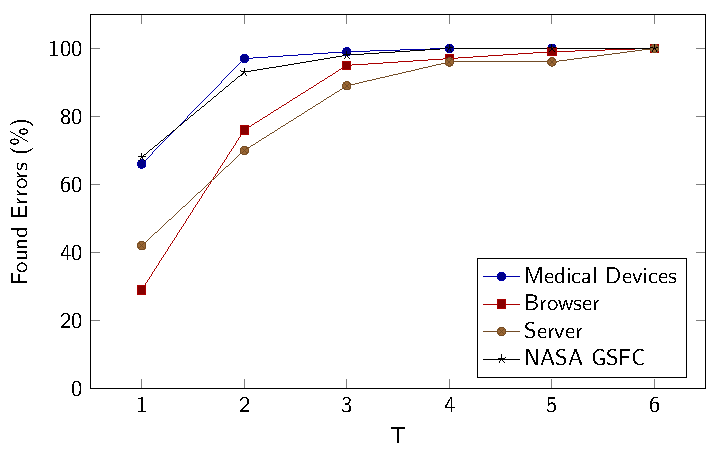
\includegraphics[width=\linewidth,page=1]{cit-plots}
		\end{exampletight}
	\mynextcolumn
		\begin{note}{Trade-Off}
			large t: high coverage (more effective)
			
			small t: low testing effort (more efficient)
		\end{note}
	\end{mycolumns}
\end{frame}
